\chapter{Patterns for Web-based IoT Applications}
\label{chapter:Patternsforweb-basedIoTapplications}

\section{RPC}
Remote Procedure Call (RPC) is one of the Inter-Process Communication methods for data exchange among threads or processes on different hosts. Unlike a local application case \cite{srinivasan1995rpc}, where the code runs all locally, RPC solves the problem of excusing codes of the whole application which is distributed cross different networks or the Internet.

RPC can be further developed into a massage pattern \footnote{http://wamp.ws/faq\#rpc} involving two roles, client and server. Usually, RPC pattern is initiated by a client, which sends an request to a remote server; The server processes based on the request, then responses to the client. An example of RPC pattern is shown in Figure \ref{fig:RPC-pattern}. The client starts its procedure sequence when the programme is running. The procedure sequence starts with Procedure 1. The client, afterwards, needs the result from Procedure 2 which locates on the Server. Thus, it sends a request to the server. The server handles the logic when the request comes, and thus it starts Procedure 2. At the moment, the Client is waiting for the result until the server responses to the client. With the result, the client can now continue to execute the next procedure, Procedure 3.  

\begin{figure}[ht]
  \begin{center}
    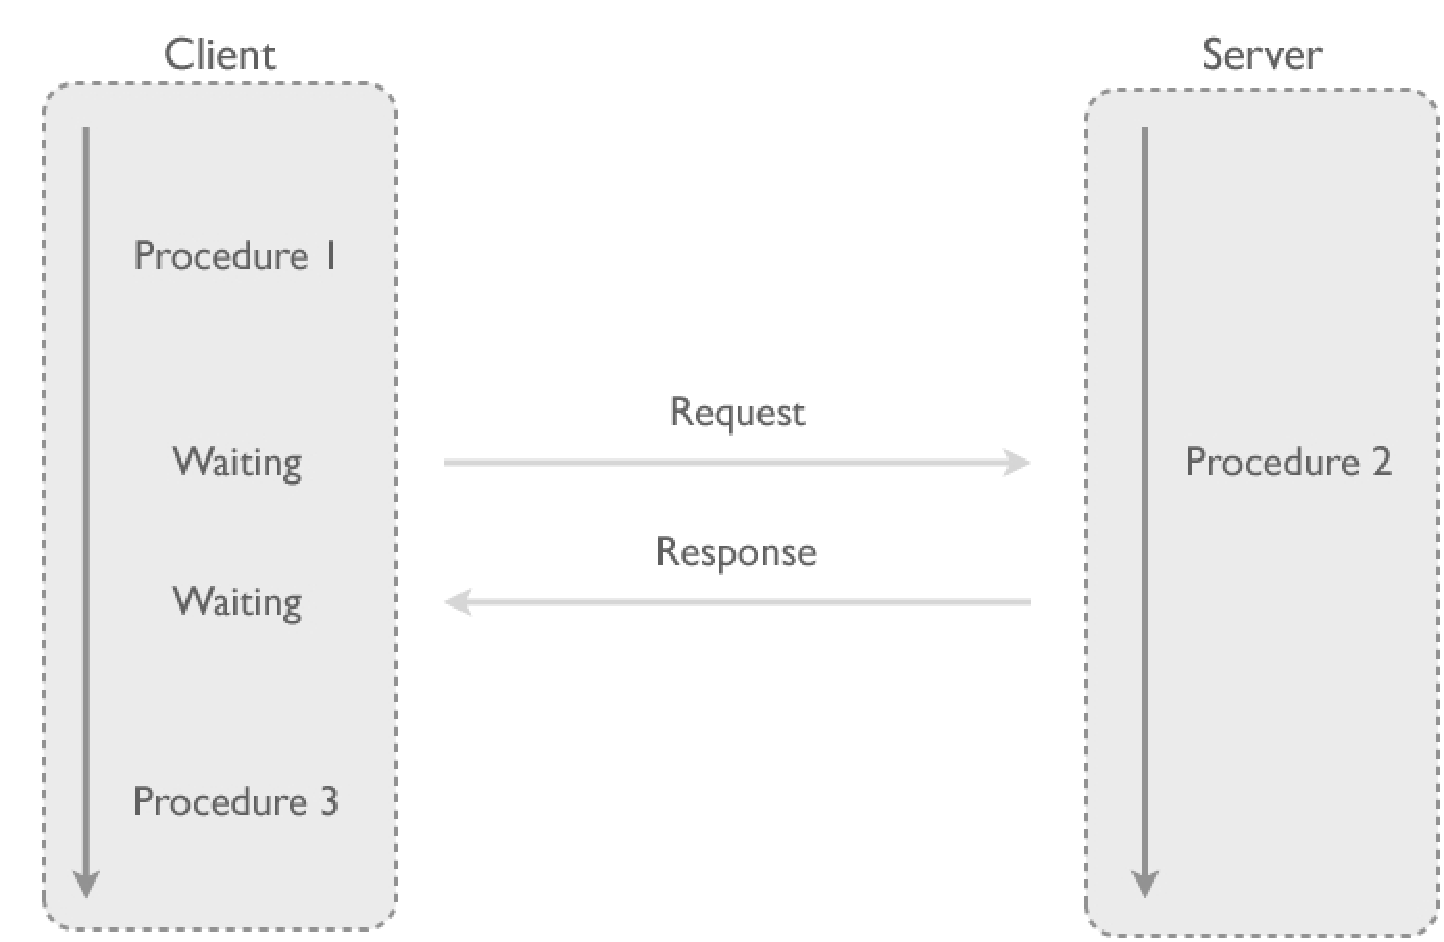
\includegraphics[width=1\textwidth]{images/RPC-pattern.pdf}
    \caption{An Example of RPC Pattern}
    \label{fig:RPC-pattern}
  \end{center}
\end{figure}

RPC is commonly used in real world scenarios. For example, Facebook, a social network web platform, provides open APIs that allows third party applications to access its data. Here, Facebook plays the role of the server(s), while the third party applications play the role of the client. When a third party application (client) sends a request to Facebook asking, e.g. a list of the user's friends, Facebook servers process the request. Facebook servers, then, response to the client, when the result, either success or error, is ready. The client can then use the list of friends to perform further procedures. 

From the perspective of IoT, RPC pattern covers one of the two most important interaction in the IoT application architecture, i.e. commanding. In the case of IoT, nodes could locate on different locations from cities to countrysides. Commanding is helpful to configure a node remotely, e.g. setting the parameters (device identification, timeout and reporting rate). As for an actuator, RPC pattern can control its action. e.g. a light actuator, or called a light switch, has the actions of on and off. With commanding, the light can, thus, be switched on or off remotely.

\section{Publish/Subscribe}

Publish/Subscribe (Pub/Sub) is one of the messages exchanges patterns. Messages are exchanged based on publishing and subscribing. A sender of a message is called a publisher. Usually, each message contains a topic. A receiver filters and receives a message by the message topic. The receiver who subscribes topics is called a subscriber. 

Pub/Sub architecture consists, usually, at least publishers, subscribers and a broker(s). The broker maps the right messages to the right receivers and exchanges messages among publishers and subscribers. Generally, there is, on one hand, no restricted boundary between a publisher and a subscriber. This means, a publisher can also be a subscriber and receives messages from other publishers; while a subscriber can also be a publisher and publishes messages with topics. On the other hand, there is no order between publishing and subscribing. This means, a publisher can publish a message with a topic without subscribing any topic; or even no one subscribes the topic. The subscriber does not have to subscribe any topic either. This refers to, if the aforementioned situation happens, then messages are , e.g., simply discarded. All the message exchanging logics, however, are handled by the broker(s). The broker(s) should specifies and implements corresponding functions to different messaging situations. 

An example of Pub/Sub pattern is shown in Figure \ref{fig:publish-subscribe-pattern}. Client 1 plays roles in both subscriber and publisher in different stages. i.e. When it subscribes topic 1, client 1 is treated as a subscriber. Client 1, however, changes to a publisher when it publishes a message with the topic (topic 1). The broker analyses the message and maps the topic to the subscribers who are interested in the topics. In this case, both Client 1 and Client 2 are interested in the topic. Hence, the broker replies the message to both of them. Client 1, and thus, changes its role to a subscriber.

\begin{figure}[ht]
  \begin{center}
    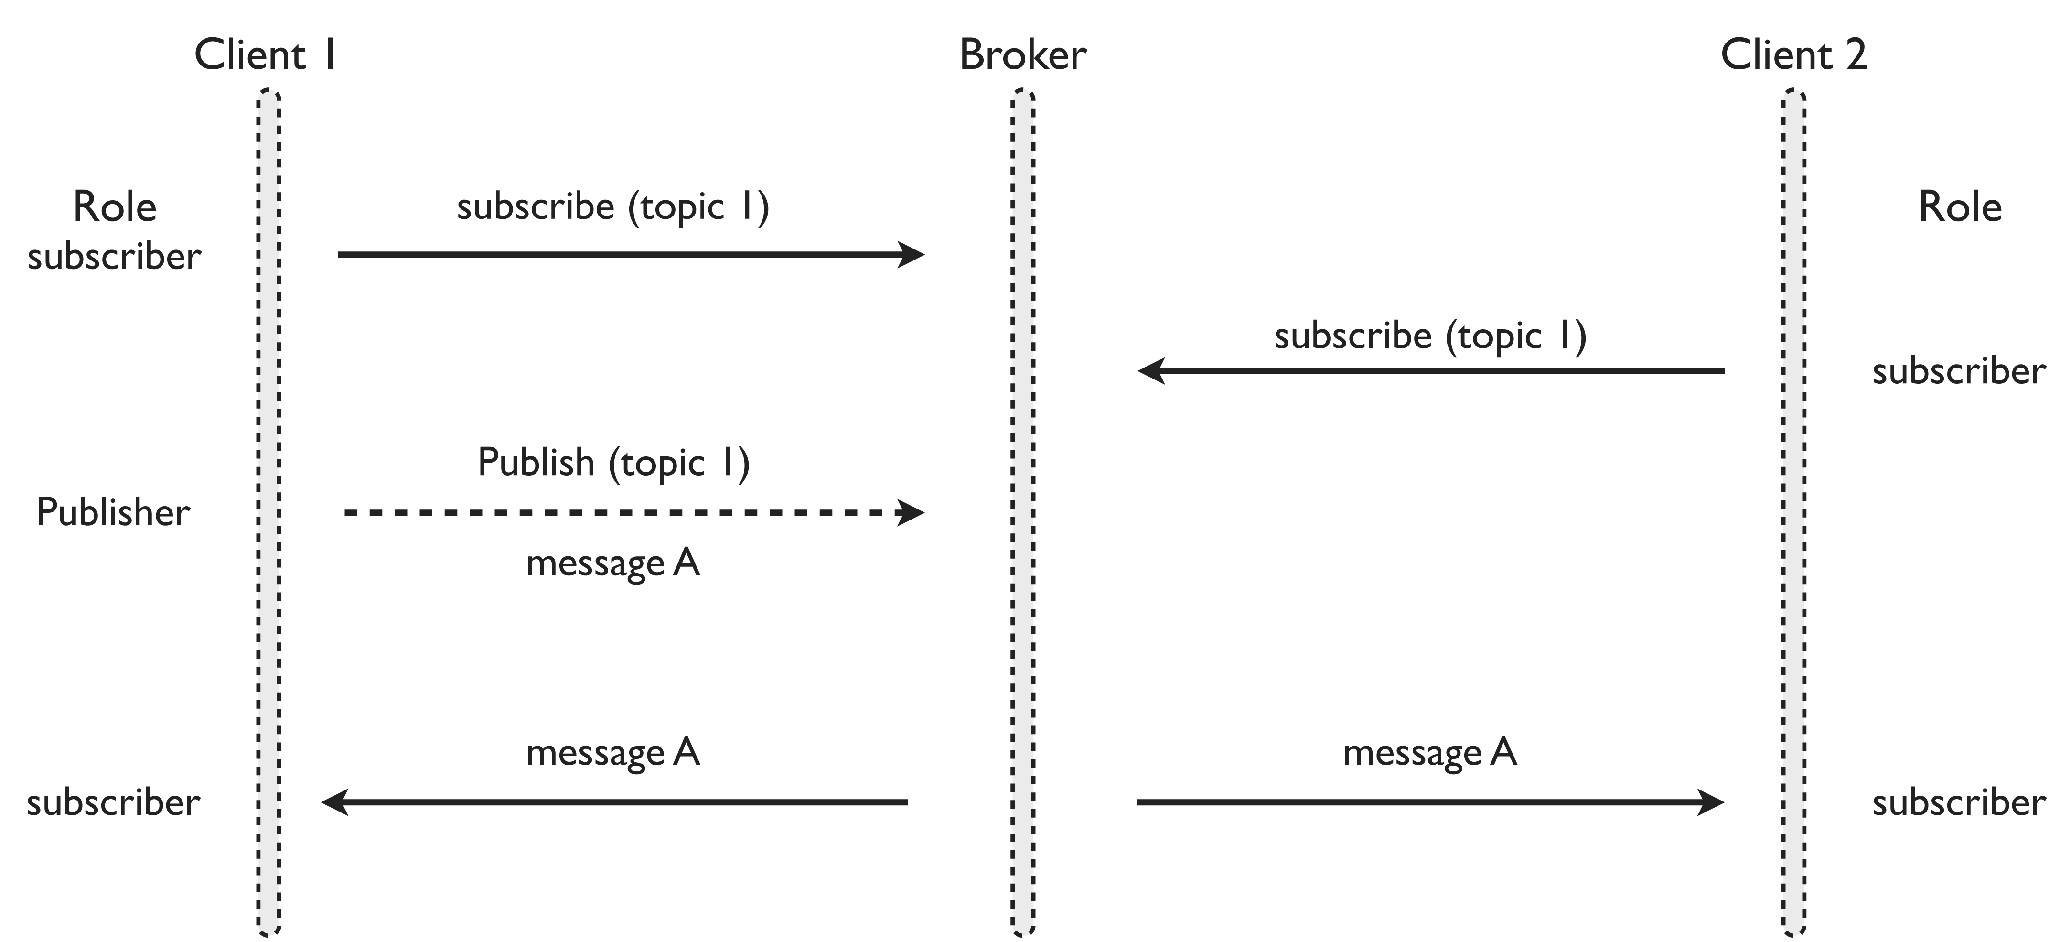
\includegraphics[width=1\textwidth]{images/publish-subscribe-pattern.pdf}
    \caption{An Example of Publish/Subscribe Pattern}
    \label{fig:publish-subscribe-pattern}
  \end{center}
\end{figure}

The concept of Pub/Sub pattern has been used in real world cases. Twitter, for example, can be treated as a real world scenario, even though the implementation might be different in Twitter. When a new user, User 1, posts a message in Twitter, usually, it will not popup on any other users' home page, but it will popup on User 1's homepage or a similar page that represents the user. This can be understood that User 1 subscribes himself, but no one subscribes him. 

User 1 can follow other users based on his interest. For example, User 1 follows User 2. User 1 will, then, receives User 2's post on User 1's homepage. Here, User 2 becomes a topic that User 1 subscribes; User 1 is the subscriber and User 2 is the publisher. Twitter, acts as a broker, handles the logic how the messages sent by User 2 delivers to User 1.

From the perspective of IoT, Pub/Sub pattern covers the other one of the two most important interaction in the IoT application architecture, i.e. notification. With notification, data can be sent interconnected, such as among nodes or from nodes to data centres. For example, one node, Node A, collects temperature data and humidity data. Node A then submits the collected data to the other node or data centre (called Node B) for the purpose of assembling. One strategy, which organises and manages the data sent by Node A, is to set the topic of the each message to the data type (i.e. temperature or humidity). Subsequently, Node B can easily categorise the data for further processing. There are, surely, other ways of exploiting Pub/Sub pattern. 

\section{Database-centric Approach}
Database-centric is a software architecture where database plays critical role. Generally, database provides fault tolerant and reliable transactions. Database-centric Approach, in IoT services, subsequently, provides a dependable mechanism to record enormous IoT data. 

An example of implementing a database-centric IoT service has been discussed in \cite{francesco2012storage}. The approach merges the features of database-centric approach with the demands of IoT services, and provides customised features for IoT services. Thus, the approach, firstly, supports heterogeneous and multimedia contents; Secondly, it provides standard APIs for standard web services, and thus the IoT data can be utilised at optimally maximum; Finally, live notification is supported and security features are applied.



